\documentclass[hyperref=colorlinks]{beamer}
\mode<presentation>
\usetheme{iclpt}
\setbeamertemplate{navigation symbols}{}
\setbeamertemplate{headline}{
\begin{beamercolorbox}[leftskip=.2cm,rightskip=.2cm,topskip=.2cm,ht=1.1cm,dp=0.1cm,wd=\textwidth]{institute in head/foot}
  
\includegraphics[height=1cm]{icl.pdf}
  \hfill
  
\includegraphics[height=1cm]{../Pics/CMS-Color.pdf}
\end{beamercolorbox}
}
\setbeamertemplate{footline}{
\begin{beamercolorbox}[ht=.55cm,dp=0.4cm,wd=\textwidth,leftskip=.3cm]{author in head/foot}%
  \begin{minipage}[c]{5cm}%
    \usebeamerfont{author in head/foot}
    \insertshortauthor 
    \insertshorttitle
    \end{minipage}\hfill%
  \insertframenumber{} / \pageref{lastframe}
  \hfill
  \begin{minipage}{6cm}
    \hfill
  \end{minipage}
\end{beamercolorbox}%
}

\usepackage{color}
\usepackage{tabularx,colortbl}
\usepackage{graphicx}
\usepackage{pdfpages}
\usepackage{feynmp}
\DeclareGraphicsRule{*}{mps}{*}{}

\title{\vspace{-0.2cm} Combination of Higgs to Invisible Direct Measurements}
%\subtitle{AN-12-403,PAS-HIG-13-013 \vspace{-0.7cm}}
\author[P. Dunne]{\underline{P. Dunne}, N. Wardle}%{D.Colling, G. Davies \underline{P. Dunne}, N. Wardle} % A.M. Magnan and A. Nikitenko Joao Pela with \\ R. Aggleton, J. Brooke: Bristol \\ C.Asawangtrakuldee, Q.Li: Peking \\ P. Srimanobhas: Chulalongkorn \\ S. Kumar, K. Mazumdar: Mumbai}
\titlegraphic{
  \vspace{-0.7cm}
%% \begin{fmfgraph*}(100,70)
%%         \fmfleft{i1,i2}
%%         \fmfright{o1,o2,o3}
%%         \fmf{fermion}{i1,v1,o1}
%%         \fmf{fermion}{i2,v2,o3}
%%         \fmf{phantom,tension=4/5}{v1,v2}
%%         \fmffreeze
%%         \fmf{photon,label=$W,,Z$}{v1,v3}
%%         \fmf{photon,label=$W,,Z$}{v2,v3}
%%         \fmf{dashes}{v3,o2}
%%         \fmflabel{$q$}{i1}
%%         \fmflabel{$q$}{i2}
%%         \fmflabel{$q$}{o1}
%%         \fmflabel{$q$}{o3}
%%         \fmflabel{$H$}{o2}
%%       \end{fmfgraph*}
}
\date{}
\begin{document}
\begin{fmffile}{feynmandiags}

%TITLE PAGE
\section{Title}
\begin{frame}
  \titlepage
  
\end{frame}

%OUTLINE
%% \begin{frame}
%%   \frametitle{Introduction}
%%   \begin{itemize}
%%   \item Decays of the Higgs boson to invisible final states are a strong indication of BSM physics
%%   \item[-] SUSY, graviscalars, etc.
%%   \item Because the final state is invisible the search must be carried out in the associated production channels:
%%   \item[-] Search for large missing transverse energy plus associated production
  
%%   \end{itemize}
%% \end{frame}

%% \begin{frame}
%%   \frametitle{Analyses}
%%   \begin{itemize}
%%   \item There are two currently approved CMS analyses searching for invisible final states of the Higgs boson.
%%   \item[-] HIG-13-013, VBF production
%%   \item[-] HIG-13-018, ZH channel where the Z decays to 2 leptons
%%   \item A further analysis, HIG-13-028, in the ZH channel where the Z decays to 2 b quarks is in progress
%%   \item An indirect limit can also be placed using the signal strength of the visible channels
%%   \item[-] Combination between direct and indirect methods is being investigated e.g. \href{https://indico.cern.ch/getFile.py/access?contribId=3&sessionId=9&resId=1&materialId=slides&confId=267834}{talk by M. Zanetti}
%%   \end{itemize}
%% \end{frame}

%% \begin{frame}
%%   \frametitle{Current Indirect Result}
%%   \centering
%%   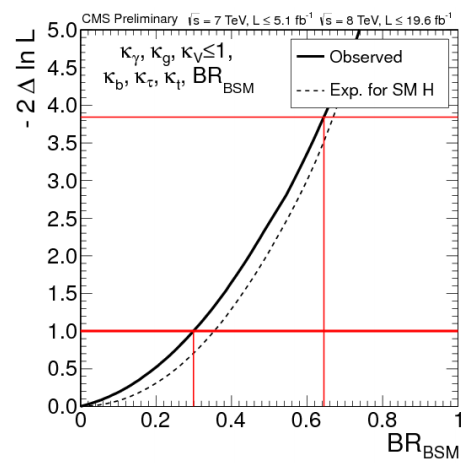
\includegraphics[height=.7\textheight]{indirectbrbsm.png}
%%   \begin{itemize}
%%   \item observed (expected) limit of 64\% (67\%) at 95\% C.L. on $BR_{inv} $ for a 125 GeV Higgs
%%   \end{itemize}
%% \end{frame}

%% \begin{frame}
%%   \frametitle{Individual Results: Direct}
%%   \centering
%%   \begin{columns}
%%     \column{.5\textwidth}
%%     \begin{itemize}
%%     \item VBF
%%     \end{itemize}
%%     \column{.5\textwidth}
%%     \begin{itemize}
%%     \item ZH
%%     \end{itemize}
%%   \end{columns}
%%   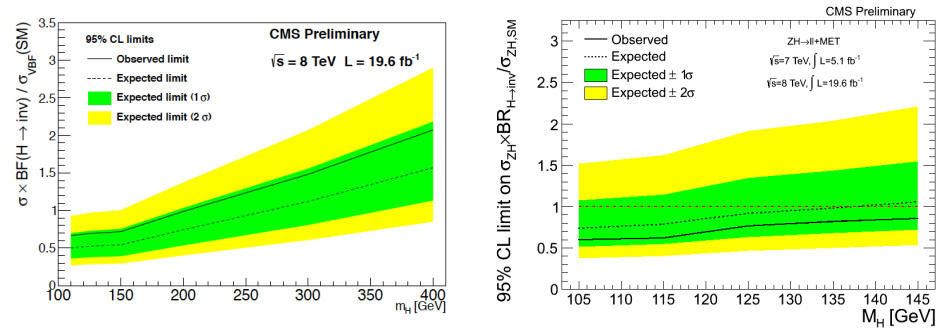
\includegraphics[width=\textwidth]{individualresults.png}
%%   \begin{columns}
%%     \column{.5\textwidth}
%%     \begin{itemize}
%%     \item observed (expected) limit of 69\% (53\%) at 95\% C.L. on $BR_{inv}$ for a 125 GeV Higgs
%%     \end{itemize}
%%     \column{.5\textwidth}
%%     \begin{itemize}
%%     \item observed (expected) limit of 75\% (91\%) at 95\% C.L. on $BR_{inv}$ for a 125 GeV Higgs
%%     \end{itemize}
%%   \end{columns}

%% \end{frame}

\begin{frame}
  \frametitle{Datacards}
  \begin{itemize}
  \item ZH analysis (cards from M. Zanetti) has datacards for 105,115,125,135 and 145 GeV
  \item VBF analysis has datacards for 110,125,150,200,300 and 400 GeV
  \item[-] The signal yield is the only Higgs mass dependent part of the datacard
  \item[-] New VBF datacards were produced for 115,135 and 145 GeV, with signal yields caluclated using method on the next slide
  \end{itemize}
\end{frame}  

\begin{frame}
  \frametitle{Signal Yield interpolation}
  \begin{columns}
    \column{.5\textwidth}
    \begin{itemize}
    \item $N_{Signal}=eff. \times acc. \times \mathcal L\sigma$
    \item Luminosity is constant
    \item Yield over cross-section is thus proportional to efficiency times acceptance
    \item Signal yields were produced at 115, 125(to cross-check), 135 and 145 GeV for the VBF channel
    \item[-] Cross-sections from LHC-HXSWG were used
    \end{itemize}
    \column{.5\textwidth}
    \centering
    \hspace{-.5cm}
    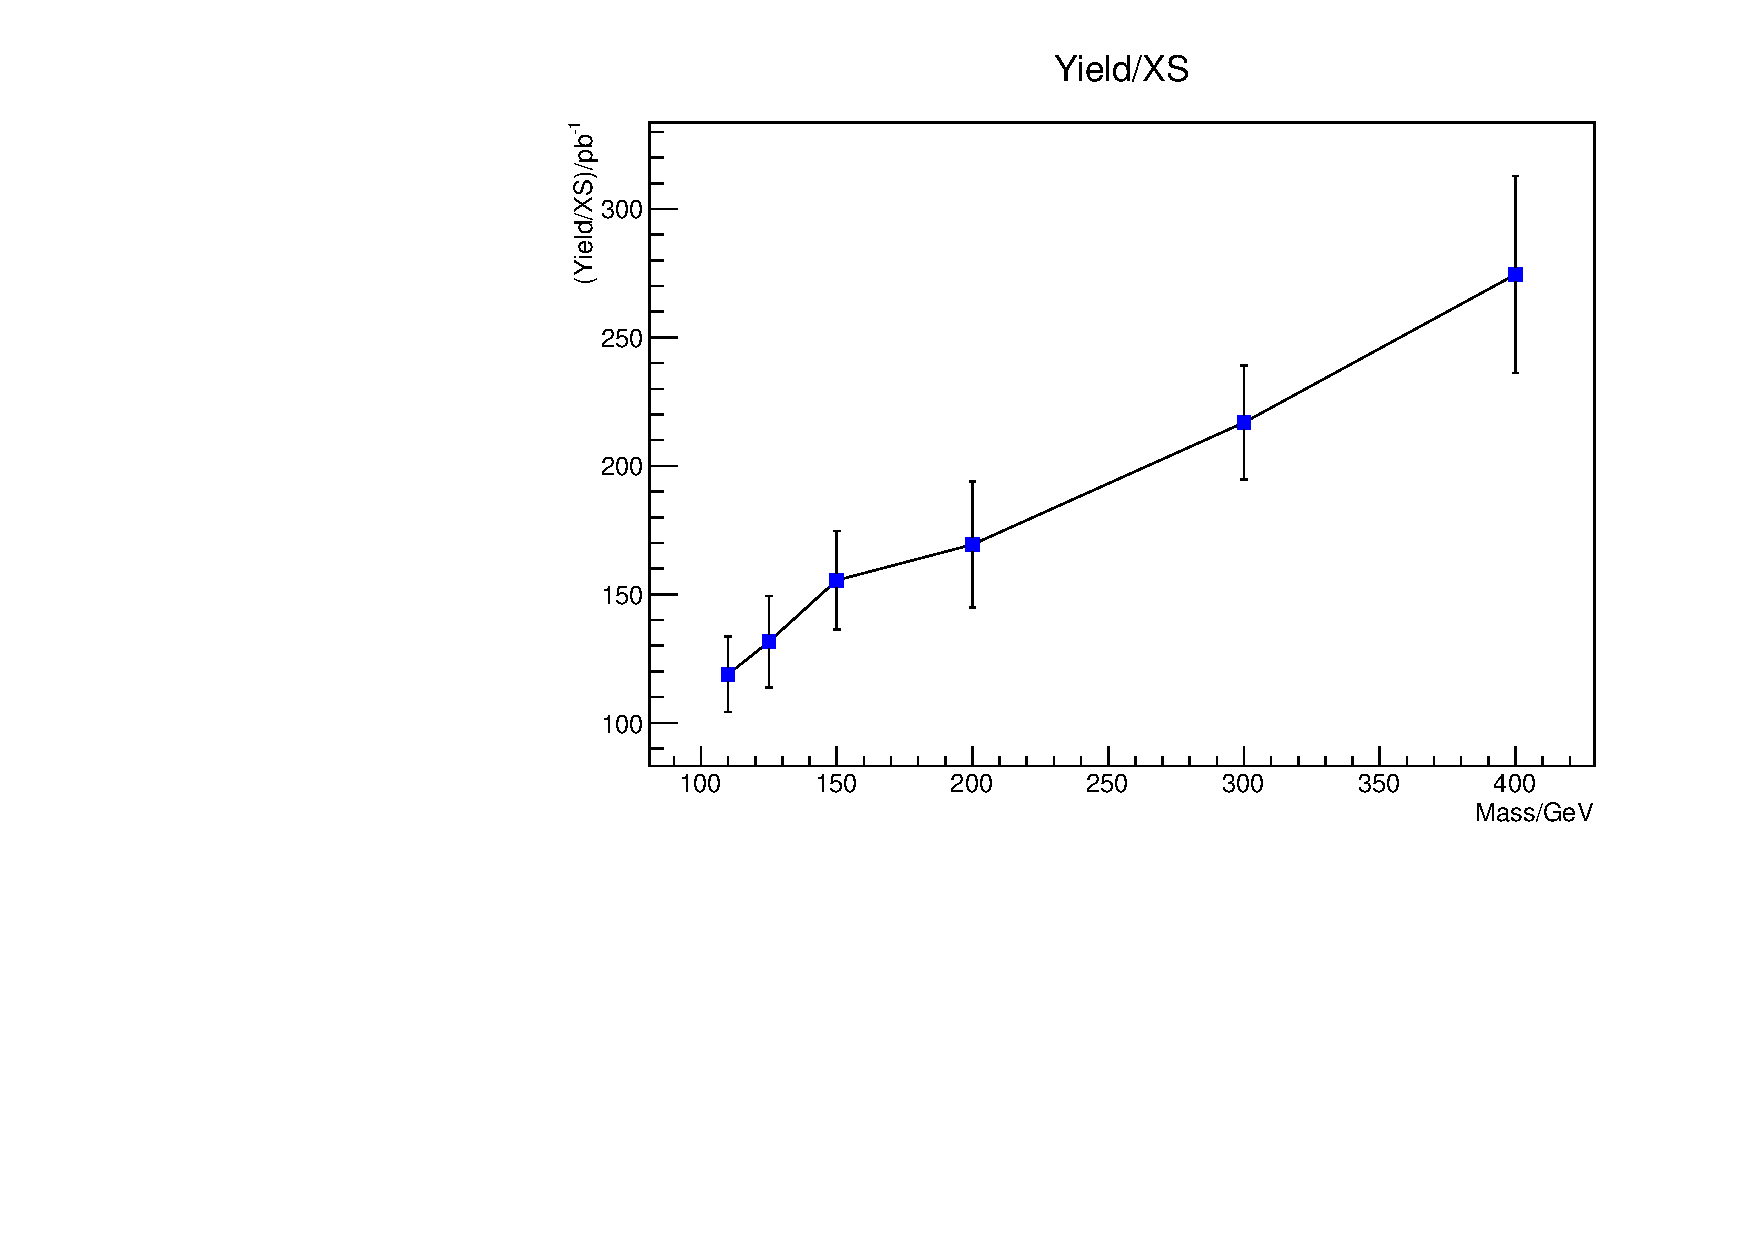
\includegraphics[clip=true,trim=0 0 0 30, width=1.2\textwidth]{yieldoverxs.pdf}
  \end{columns}
\end{frame}

\begin{frame}
  \frametitle{Combination Method}
  \begin{itemize}
  \item The cards for the two approved analyses were combined using the standard Higgs combination tool
  \item The luminosity uncertainties were considered correlated between the analyses
  \item All other uncertainties were considered not to be correlated between analyses
  \item[-] The VBF analysis datacard does not separate out individual sources of error so JES/R correlations cannot be taken into account without more information
  \end{itemize}
\end{frame}
    
\begin{frame}
  \frametitle{Results}
  \centering
  \vspace{-.2cm}
  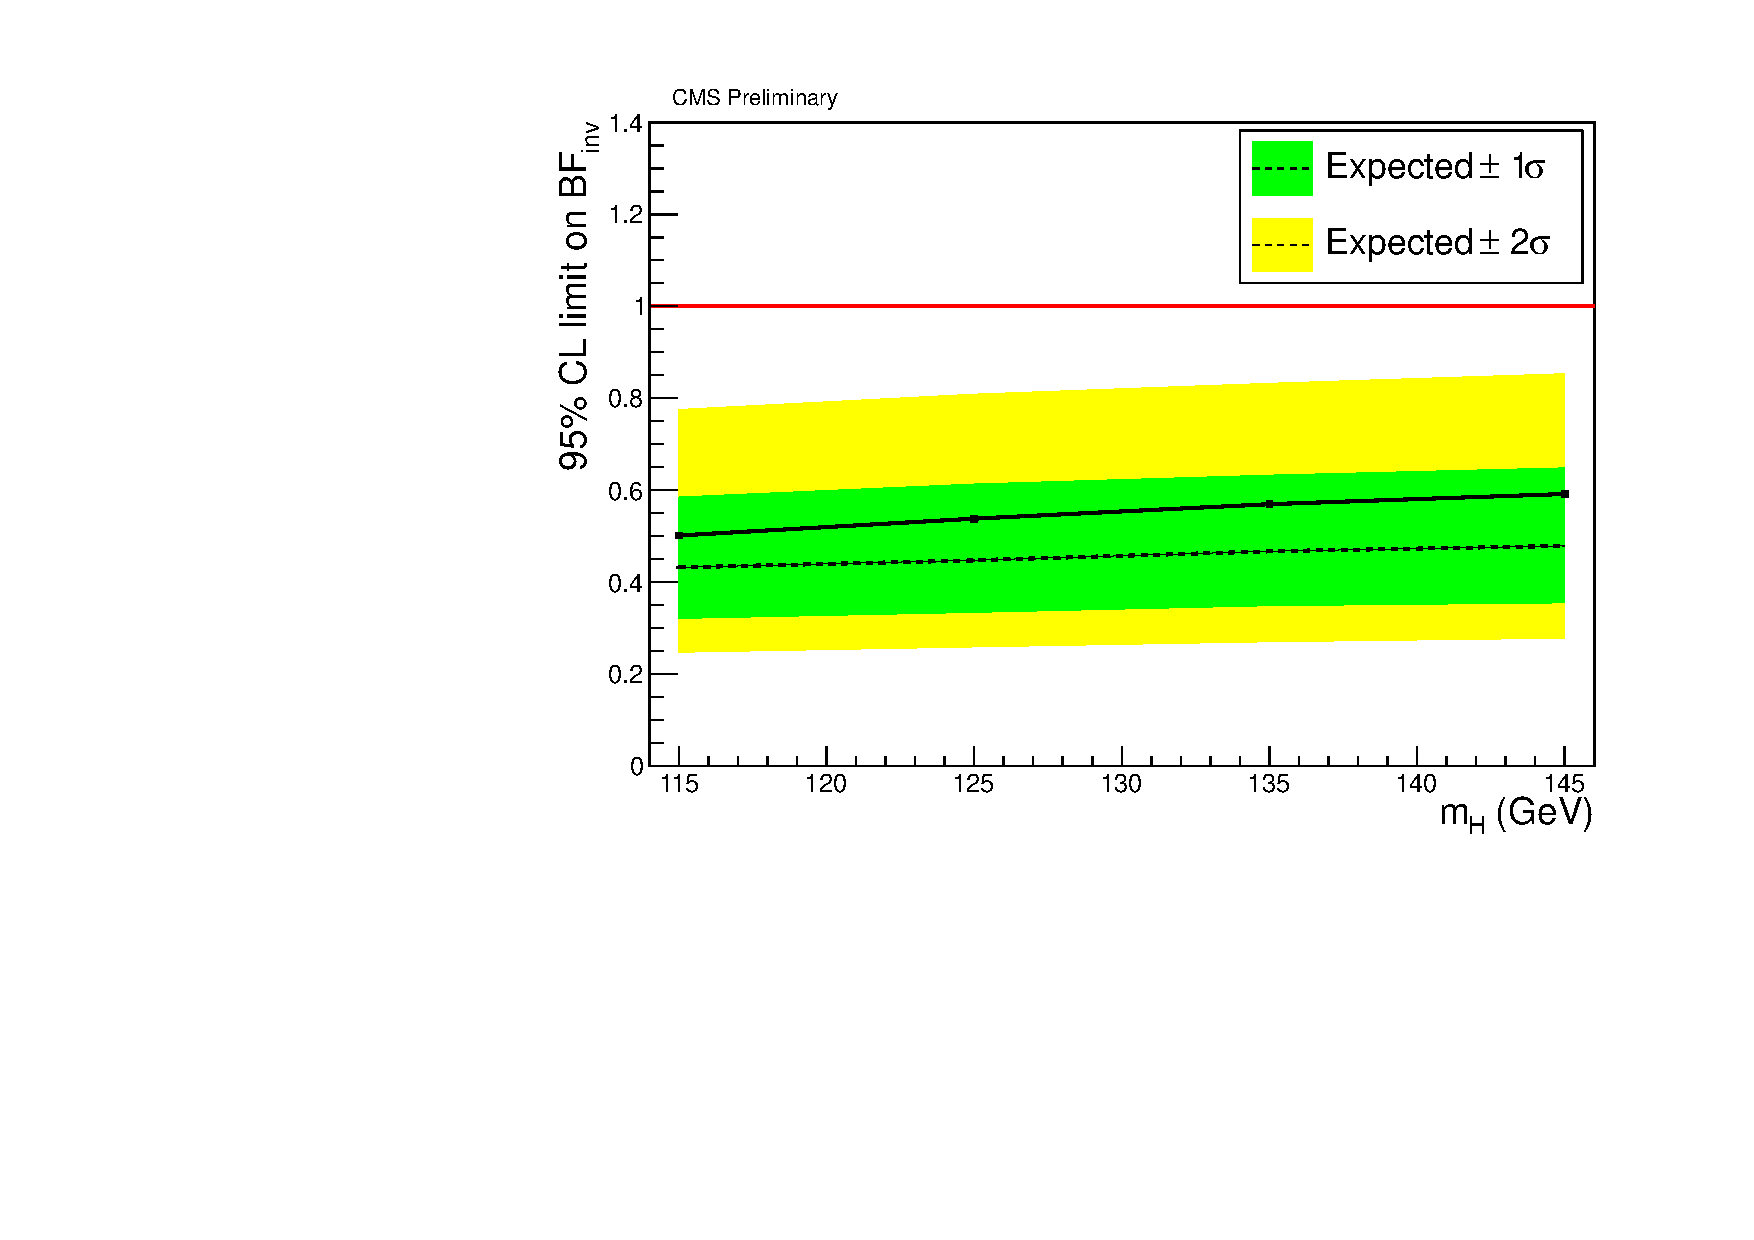
\includegraphics[clip=true,trim=0 5 0 20, width=.8\textwidth]{invlimit.pdf}
  \vspace{-.3cm}
  \begin{itemize}
  %% \item The expected limit is found to be: 46\%
  %% \item[-] The 68\% C.L. band on the expected limit is 34-62\%
  %% \item The observed limit is 53\%
  \item Observed (expected) limit at 125 GeV is 54(45)\%
  \item Consistent with number from M. Zanetti's talk 56(47)\%
  \end{itemize}
\label{lastframe}
\end{frame}
    
%% \begin{frame}
%%   \frametitle{Conclusions}
%%   
%%   \begin{itemize}
%%   \item The results of HIG-13-013 and HIG-13-018 have been combined using the standard Higgs combination tool
%%   \item The result is compatible with the SM at the 1$\sigma$ level
%%   \item The combined result gives strongest direct limit on the invisible branching fraction of the SM Higgs
%%   \item[-] Values at 125 GeV in agreement with that shown by M. Zanetti
%%   \end{itemize}
%% \end{frame}

%% \begin{frame}
%%   \frametitle{Backup}
%% \end{frame}

%% \begin{frame}
%%   \frametitle{Previous Limits}
%%   \begin{itemize}
%%   \item Current CMS limits on $BR_{inv}$ for a 125 GeV Higgs boson are:
%%   \item[-] VBF: observed (expected) limit of 69\% (53\%) at 95\% C.L.
%%   \item[-] ZH: observed (expected) limit of 75\% (91\%) at 95\% C.L.
%%   \item[-] CMS indirect limit, from visible channels: observed (expected) limit of 64\% (67\%) at 95\% C.L.
%%   \item ATLAS also produce an indirect limit and a limit in the ZH channel:
%%   \item[-] Indirect limit 60\% (no expected limit given)
%%   \item[-] ZH: observed (expected) 65\% (84\%)    
%%   \end{itemize}
%% \end{frame}

%% \begin{frame}
%%   \frametitle{VBF Cross-sections}
%%   \centering
%%   \begin{tabular}{|l|c|}
%%   \hline  
%%   Mass/GeV & $\sigma/pb$ \\
%%   \hline  
%%   110 & $1.809 \pm 0.048$\\
%%   115 & $1.729 \pm 0.046$\\
%%   125 & $1.578 \pm 0.042$\\
%%   135 & $1.448 \pm 0.038$\\
%%   145 & $1.333 \pm 0.035$\\
%%   150 & $1.280 \pm 0.033$\\
%%   200 & $0.869 \pm 0.023$\\
%%   300 & $0.441 \pm 0.011$\\
%%   400 & $0.254 \pm 0.007$\\
%%   \hline  
%%   \end{tabular}
%% \end{frame}

 \end{fmffile}
\end{document}

